% Generated by reproduction/framework_experiments/build_manuscript_assets.py.
\subsection{路线 B：预测、跟踪与参考同步}
\label{num:route-b}
施加控制之前，从相同初态分别用细步长 RK4 积分，并以 $h_*$ 检验保守预测。标称 $h_0$ 的状态 RMS 为 $8.04072\times10^{-6}$；换用拟合的 $\widehat h$ 后，误差为 $1.35426\times10^{-10}$。这一比较检验所选保守扰动的恢复。随后控制实验冻结 $\widehat h$，将其参考初始化在路线 A 的初态，并使实际受控对象偏移 $(0.0045,0.004,0,0)$。增益 $\kappa_p=1$ 和 $\kappa_d=2$ 使式~\eqref{struct:route-b-oracle} 所定义的真值参数对照控制律对应的位置误差动力学达到临界阻尼。包括真值参数对照在内的四个控制组均采用同一冻结参考。

实际状态与参考状态合并为一个八维中点系统进行积分。
另保留第二条独立积分的 RK4 参考，仅用于评估。
记 $x_k$ 为实际状态，$\bar x_k$ 为同步中点参考，
$x_{\mathrm{ref}}(\tau_k)$ 为独立参考，则
\begin{equation}
 x_k-x_{\mathrm{ref}}(\tau_k)
 =(x_k-\bar x_k)+
   (\bar x_k-x_{\mathrm{ref}}(\tau_k)).
 \label{num:reference-split}
\end{equation}
第一项衡量对实际实现参考的同步误差；第二项保留该参考自身的积分误差。
表~\ref{num:b-table} 同时报告这两种口径。

\begin{table*}[t]
\centering
\caption{路线 B 在 $\Delta=0.001$ 时的状态均方根误差。
“独立”指同一冻结 $\widehat h$ 的小步长 RK4 参考；
“同步”指增广中点系统中的参考分量。}
\label{num:b-table}
\begin{tabular}{lccc}
\toprule
控制方式 & 独立，$[0,20]$ & 独立，$[10,20]$ & 同步，$[10,20]$\\
\midrule
无控制 & $2.55875\times10^{-2}$ & $3.41583\times10^{-2}$ & $3.41580\times10^{-2}$ \\
阻尼补偿 & $6.02185\times10^{-3}$ & $6.02249\times10^{-3}$ & $6.02060\times10^{-3}$ \\
学习跟踪 & $1.58912\times10^{-3}$ & $2.26767\times10^{-5}$ & $8.55100\times10^{-7}$ \\
真值参数对照跟踪 & $1.58912\times10^{-3}$ & $2.26767\times10^{-5}$ & $8.55090\times10^{-7}$ \\
\bottomrule
\end{tabular}
\end{table*}

学习控制器相对于独立参考的全时窗均方根误差为 $1.58912\times10^{-3}$，
其中包含预先设定的启动误差。
在 $10\leq\tau\leq20$ 上，该值降为 $2.26767\times10^{-5}$，
而同步均方根误差为 $8.55100\times10^{-7}$。
在终点，同步误差为 $2.98323\times10^{-10}$，但相对于独立参考的误差为 $2.96937\times10^{-5}$。
中点参考的最大误差为 $2.96936\times10^{-5}$；将中点步长减半后，该误差缩小 $3.999984$ 倍。
因此，近乎完美的同步可以与已经分辨出的二阶参考相位误差同时存在。
不能将同步误差报告为对连续参考运动的逼近精度。

另一项检查将真值参数对照的跟踪误差，与其线性误差方程的 Cayley 更新进行比较。
最大差值为 $1.0040\times10^{-15}$。
这验证了增广中点耦合，但并未使稳定跟踪闭环成为哈密顿系统。
实验也说明了单独补偿阻尼为何不足以实现此目标：它不能消除预先施加的初始位置偏差。

\begin{figure*}[t]
\centering
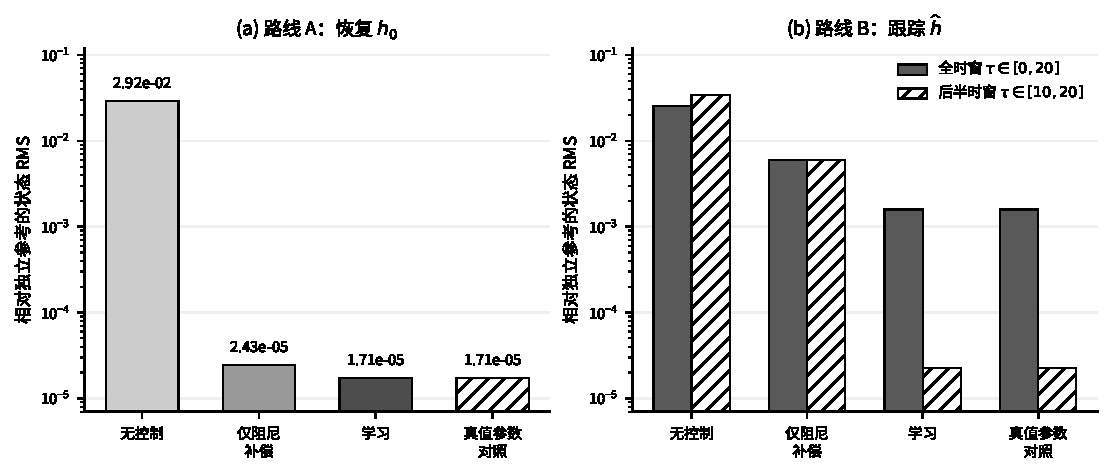
\includegraphics[width=\textwidth]{figures/new_baseline_results.pdf}
\caption{采用独立保守参考的新基准比较。
(a) 路线 A 从相同初态恢复 $h_0$。
(b) 路线 B 从非零初始偏差出发，跟踪冻结的 $\widehat h$ 轨迹。
全时窗与后半时窗误差揭示了跟踪暂态。
两个面板使用不同参考对象，因此柱高不能用于对两条路线作优劣排序。}
\label{num:results}
\end{figure*}

\subsection{路线 B 预测与跟踪协议}
\label{sx:route-b}
路线 B 脚本重新生成同一组训练与验证数据，
并检查其新拟合的系数向量与路线 A 向量的差异是否在 $10^{-13}$ 以内。
随后针对 $h_0$、$\widehat h$ 和 $h_*$ 分别计算三条保守轨迹，
采用 RK4 步长 $0.00025$，从共同初态积分至 $\tau=20$。
预测误差将 $h_0$ 和 $\widehat h$ 与 $h_*$ 比较；
后者是合成真值，而非独立物理数据。
对 $\widehat h$ 和 $h_*$ 参考，均另用 RK4 以步长 $0.0005$ 计算进行核查。

反馈控制的参考是冻结的保守 $\widehat h$ 流，
初态为 $(0.09,0.08,0.015,-0.01)$。
实际初态为 $(0.0945,0.084,0.015,-0.01)$。
位置偏差分别为参考各位置坐标的 $5\%$，动量偏差为零。
在无量纲时间下，增益取 $\kappa_p=1$、$\kappa_d=2$。
无控制、基于拟合参数的仅阻尼补偿、学习跟踪和真值参数对照跟踪组均使用同一参考。
学习指令与真值参数对照指令分别对应式~\eqref{struct:route-b-control} 和式~\eqref{struct:route-b-oracle} 中的不同控制律；
真值参数对照使用真实受控对象系数进行抵消，但保留拟合参考轨迹。

四个实际状态变量与四个参考变量共同构成八维中点求解，
Newton 设置与式~\eqref{sx:newton-stop} 相同。
独立 RK4 轨迹不输入该控制器，
仅在计算后用于报告式~\eqref{num:reference-split} 中的积分误差分量。
另一次计算将中点步长减半至 $0.0005$；
实际状态在共同时间点处的最大差值为 $2.22701\times10^{-5}$，
参考误差缩小 $3.999984$ 倍。
在记录的检查中，解析增广 Jacobian 与有限差分的最大差异为 $3.6902\times10^{-11}$。
这些有限差分是实现诊断，不能替代已经推导的 Jacobian。

对于真值参数对照，初始动量误差向量为零，连续误差满足
$e_X(\tau)=(1+\tau)e^{-\tau}e_X(0)$ 和
$e_Y(\tau)=-\tau e^{-\tau}\mathsf N^{-1}e_X(0)$。
还将离散误差与独立构造的该线性系统 Cayley 更新进行比较。
这一比较利用已知误差方程检验反馈与参考之间的耦合。

\subsection{跟踪敏感性与合并保留图表}
\label{xtr:shared-results}
五个阻尼设置使用与补充材料第~\ref{sx:damping}~节恢复实验相同的重新生成观测和重新拟合结果。跟踪实验持续 $\tau=10$，中点步长为 $0.002$，独立 RK4 步长为 $0.00025$；跟踪后半时窗为 $[5,10]$。这里对每个声明阻尼值独立拟合，并非让一个冻结控制器面对未知变化阻尼。下表保留两种目标，以明确显示它们不同的时间窗。

\begin{table*}[t]
\centering
\caption{阻尼扫描中相对于独立参考的状态均方根误差。
两条路线使用不同的目标哈密顿量与时间窗口。}
\label{sx:damping-errors}
\begin{tabular}{rcccc}
\toprule
$\zeta_1^{\mathrm{d}}$ & A 无控制，$[0,10]$ & A 学习，$[0,10]$ & B 无控制，$[5,10]$ & B 学习，$[5,10]$\\
\midrule
$0$ & $3.77362\times10^{-5}$ & $3.42885\times10^{-5}$ & $6.02444\times10^{-3}$ & $1.09567\times10^{-4}$ \\
$0.01$ & $6.73657\times10^{-3}$ & $3.42885\times10^{-5}$ & $3.71321\times10^{-3}$ & $1.09567\times10^{-4}$ \\
$0.025$ & $1.59501\times10^{-2}$ & $3.42885\times10^{-5}$ & $1.62063\times10^{-2}$ & $1.09567\times10^{-4}$ \\
$0.05$ & $2.92396\times10^{-2}$ & $3.42885\times10^{-5}$ & $3.42497\times10^{-2}$ & $1.09567\times10^{-4}$ \\
$0.1$ & $4.97374\times10^{-2}$ & $3.42885\times10^{-5}$ & $6.13727\times10^{-2}$ & $1.09567\times10^{-4}$ \\
\bottomrule
\end{tabular}
\end{table*}

\begin{figure*}[t]
\centering
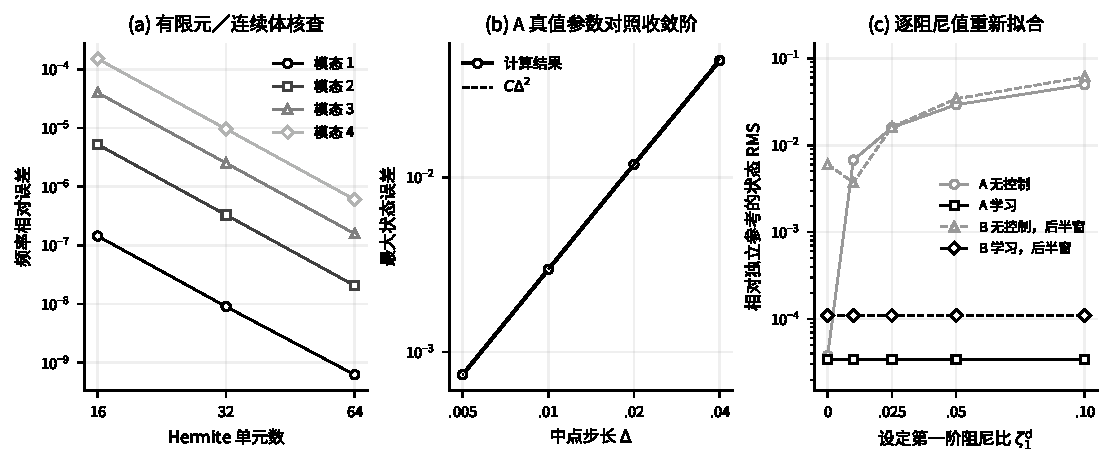
\includegraphics[width=\textwidth]{figures/new_baseline_verification.pdf}
\caption{根据随附 JSON 记录进行的独立数值核查。(a) 前四阶有限元频率收敛至连续体端点行列式的根。(b) 相对独立 RK4 参考，路线 A 真值参数对照误差以二阶收敛。(c) 每个阻尼设置均先重新拟合，再评价两条路线；A 使用完整 $[0,10]$ 时窗，B 使用后半 $[5,10]$ 时窗。连线仅连接已测试设置，不表示额外仿真或统计区间。}
\label{num:verification}
\end{figure*}
\begin{table*}[t]
\centering
\caption{补充学习跟踪实验中的采样局部磁需求。这是理想指令需求，并非硬件能力测量。}
\label{xtr:port-table}
\begin{tabular}{lcccc}
\toprule
实验 & $\max|B_y|$ (mT) & $\max|B|$ (mT) & $\max\|\nabla B\|_2$ (T/m) & $\max|F_y|$ ($\mu$N)\\
\midrule
B：学习 & $2.197941$ & $30.080408$ & $0.03453753$ & $0.611950$ \\
\bottomrule
\end{tabular}
\end{table*}
